\section{Adam Stajek\item \item }
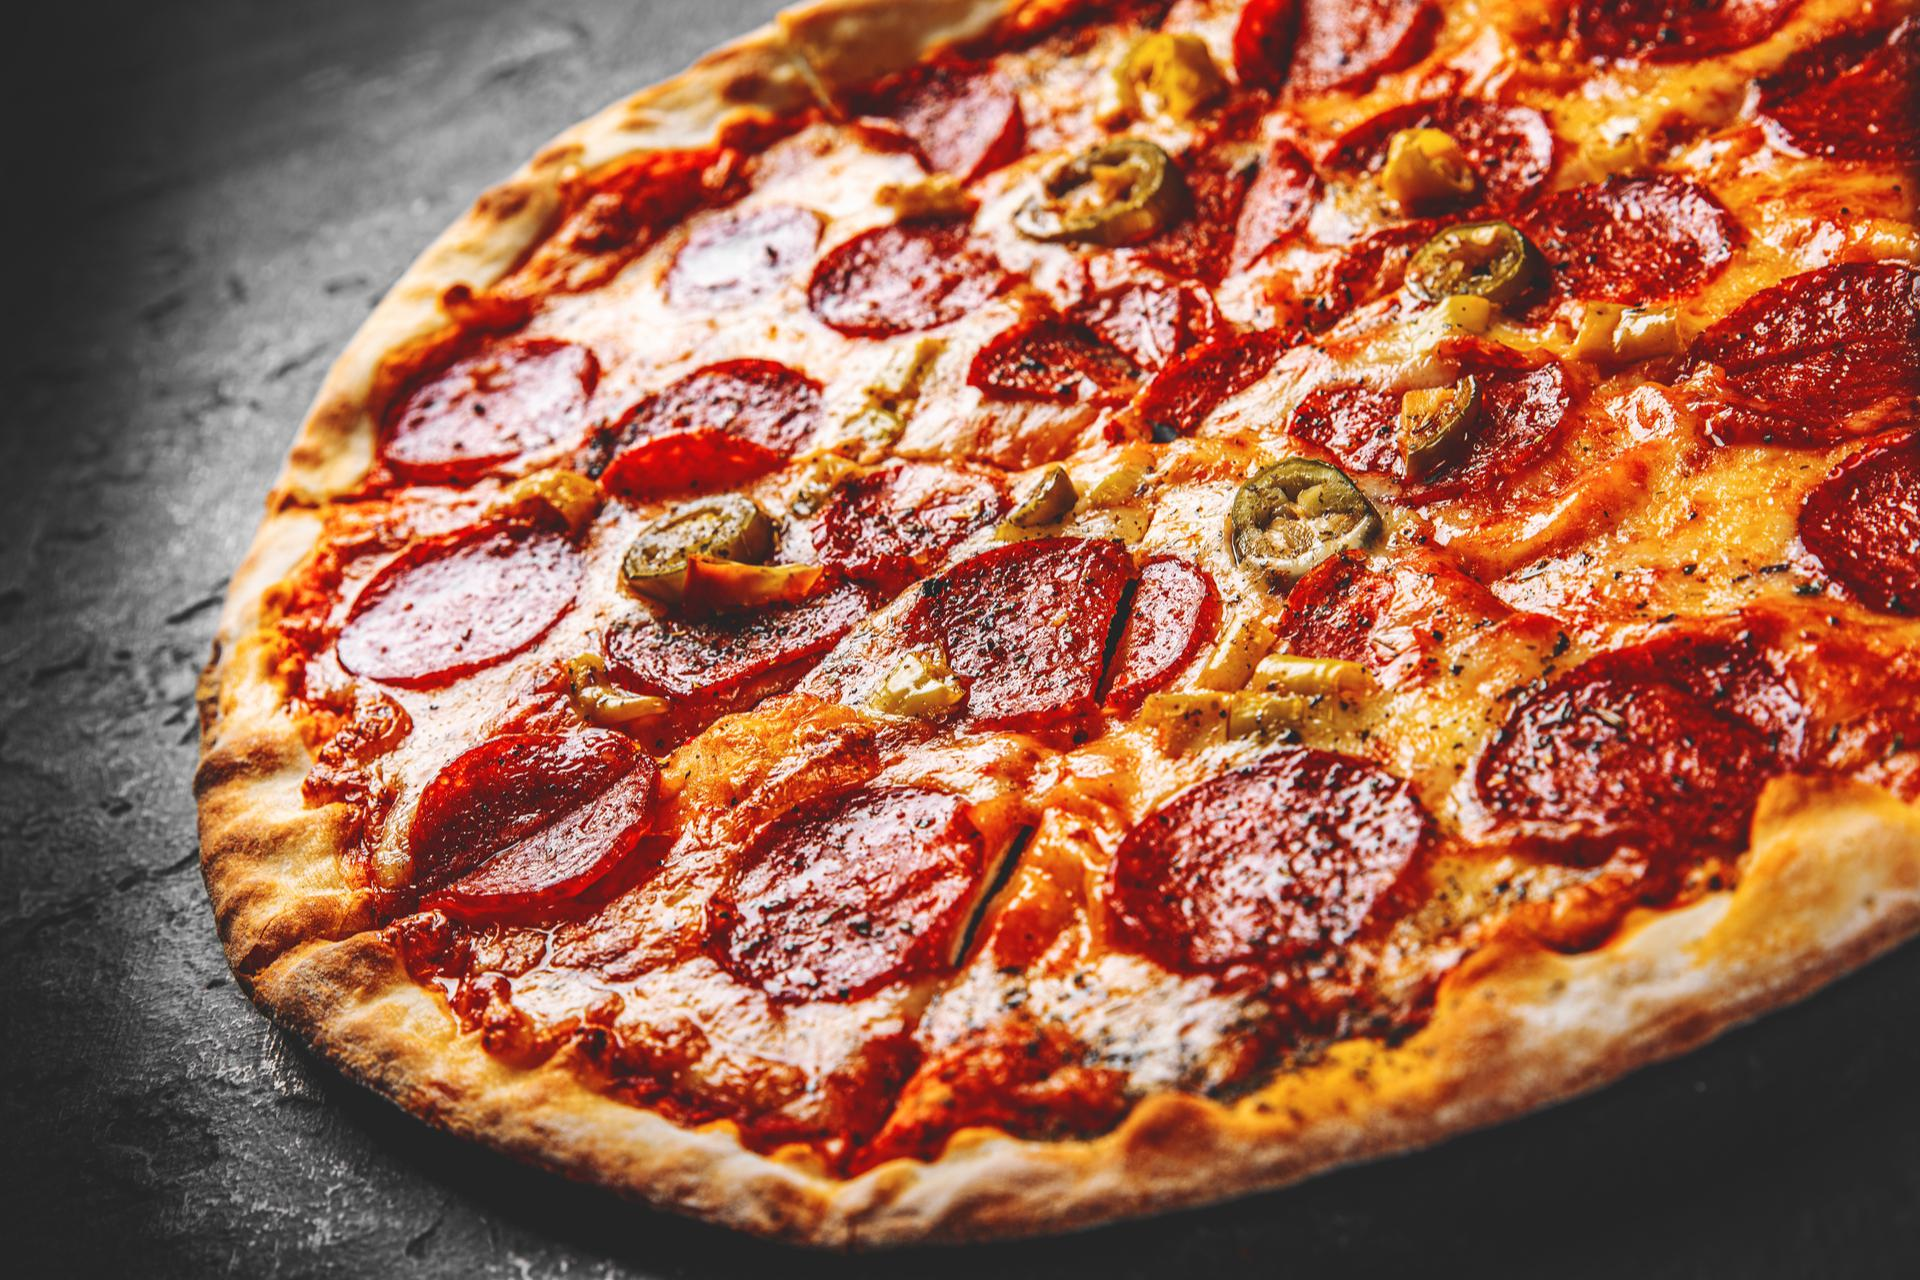
\includegraphics[width=5cm, height=4cm]{pictures/pizza.jpg} 
\newline
wzór na obliczenie pola pizzy: \(P= \pi r^2\)
\newpage
Kocham:
\begin{itemize}
  \item AGH
  \item Samogłoski
  \item Informatykę
\end{itemize}
Nie kocham:
\begin{enumerate}
  \item Pizzy z ananasem
  \item Ostrowca Świętokrzyskiego
  \item Staszica
\end{enumerate}

\newline

\begin{table}
\label{tabela}
\begin{tabular}{|l|l|l|l|l|}
\hline
a & b & c & d & e \\ \hline
f & g & h & i & j \\ \hline
k & l & m & n & o \\ \hline
p & t & d & t & u \\ \hline
\end{tabular}
\end{table}

Studia na kierunku \textbf{Informatyka i systemy inteligentne} wyposażają w wiedzę i praktyczne umiejętności z zakresu informatyki oraz sztucznej inteligencji i przygotowują do tworzenia i projektowania rozwiązań informatycznych wykorzystujących i integrujących różne systemy inteligentne. W programie studiów uwzględniono przedmioty informatyczne, matematyczne oraz fizyczne. Kształcenie na tym kierunku to jednak głównie przedmioty związane z programowaniem, a także \underline{inżynierią oprogramowania}. \par Student zdobywa kompetencje dotyczące języków i technik programowania, algorytmiki, złożoności obliczeniowej, baz danych, analizy danych oraz analizy procesów biznesowych. Przygotowuje się do projektowania, testowania i wdrażania systemów informatycznych, budowy interfejsu użytkownika, systemów operacyjnych oraz sieci komputerowych. Poznaje także takie zagadnienia, jak uczenie maszynowe, sztuczna inteligencja, programowanie inteligentnych systemów wbudowanych oraz projektowanie złożonych systemów informatycznych, co w efekcie pozwala mu na realizację zadań związanych z \emph{wytwarzaniem oprogramowania}. \newline
\newline
Pamiętaj o tabeli na stronie \pageref{tabela} \newline